\documentclass[12pt]{article}

\usepackage{tabularx}
\usepackage{pdflscape}
\usepackage{float}
\usepackage{graphicx}

\newcommand{\mypath}{./figures/}
\graphicspath{\mypath}


\title{World Robotic Sailing Championship 2019 \\
Notice of race and competition rules \\v1.1}
\date{\today}

\begin{document}
\maketitle
% GOALS:
% - Scoring based on data, measurable success
% - KISS -> simplify as far as possible
% - Additive success: No loss of all points, generally no loss of points!
% - clear and unambiguous: Don't assume things are implied, avoid formulations
%   that may lead to rule discussions.

\section{Introduction}

The World Robotic Sailing Championship 2019 will be organized during August 25th – 29th in Ningbo, China.
The World Robotic Sailing Championship will be followed by the International Robotic Sailing Conference that will be held on August 30\textsuperscript{th} in Ningbo, Zhejiang Province, China.
The organizing committee invites teams from any organization, including private individuals, schools, colleges, universities and companies, to enter the competition.
Each team competes with one boat; the team members can be shared among different teams.
The championship will be organized in 4 challenges, each one tentatively allocated to a single day. 


\section{Classes}

The only restriction on the participating ships in the WRSC is that no electricity or fuel can be used as the energy source.
The teams must be able to clearly demonstrate this to the race committee.
Vessels may use any type of hull (mono or multi) and any type of rig, with one or more soft or rigid sails.
The beam of multi-hulls should not exceed their LOA (length overall, maximum length of the hull measured parallel to the waterline) and the maximum draft of any boat should be limited to 2 m.
Hydrofoils are allowed. 
Sails and appendages may be changed between challenges. 
There is only one class in this year's competition. 

\section{Liability and Safety}
All sailing robots must be controllable by a designated human helmsman
throughout all events. The responsibility for avoiding any collision, 
damage or personal injuries will rest solely with the respective teams. 
The organizers will not assume any liability with respect to third party
damages, personal injuries or environmental contamination resulting from any
activity of a team participating in the WRSC. All teams are responsible for 
their own safety during the event and the decision to participate in the 
competitions is of the exclusive responsibility of the team members.
Before being allowed to compete, each team has to register a person of contact
who will be held responsible for any damage, injury or environmental
contamination resulting from any activity of the team, including the 
operation of their vessel.

All sailing boats will be under the supervision of support vessels provided by the
organization.
All people on board of a support vessel must follow the safety instructions of the driver 
and must provide their own personal floatation device which must be worn at all times 
while on or near the water. We aim to allow at least one member per team on a support vessel, 
however the organisers reserve the
right to manage the fleet of support vessels, and can refuse access to the support
vessels for any reason.
All team members must follow the instructions of the competition
organisers, the support vessel crew, and the activity centre personnel. The organizers
reserve the right to refuse access to restricted areas.
For safety reasons, the race area may be confined to a region delimited by 4
marks. 


  \begin{figure}[H]
    \centering
    \includegraphics[width=0.7\textwidth]{2019_area}
    \caption{The approximate race area reserved for WRSC}
    \label{fig:competitionarea}
  \end{figure}

  Figure \ref{fig:competitionarea} shows approximately the area requested for WRSC that may be subject to last
minute adjustments.


\section{Collisions and Right of Way}
Autonomous boats have right of way over manually controlled boats. In the event
of a potential
collision, then COLREGs rules must be followed (for example, a boat on a
starboard tack has
right of way, etc). However, all competitors must take appropriate actions to
avoid collisions
and having right of way is not an acceptable excuse for allowing a collision to
take place.
Remote control is allowed to avoid imminent collisions for the boat with no 
right of way. Alternatively, a collision may also be
prevented by manually holding the boat with no right of way, but ensuring that 
its position and heading is maintained until the risk of collision has passed. 
In the case a boat gets entangled with a buoy or any other
floating debris (seaweed, lines, fishing nets, etc) it can be assisted manually,
as long as no advantage is given to the boat and the required safety boat has
not higher priority tasks.

Any remote controlled or manual measures during a challenge must be
communicated to the race committee directly after the challenge.

\section{Remote control}
All teams are required to be able to take over remote-control of their boats
through a wireless connection (WiFi, RC, \ldots). The country specific 
regulations on wireless communication must be obeyed, e.g. Wifi boosters beyond
the allowed limits may not be used.
Should the race committee have doubts about the remote controllability it may
ask for a demonstration and restrict participation in challenges.

Remote control is allowed to transport competing vessels to the challenge area,
but must be switched off several metres from the start line, with the vessel
facing away from the start line.


\section{Scoring}
The WRSC is organized in 4 challenges scheduled for each day of the event: Fleet Race, Station Keeping and Avoidance, Collaborative Area Scanning and Hide and Seek. 
The scoring for each challenge will be based on the real-time positioning track uploaded by the tracker sorted from the first to the Nth (N = team number). 
In each challenge, the team that completed the challenge target ranked first in the project with a score of 1.0. The second place is awarded 1.2 points, the third place is awarded 1.4 points, so on so forth. 
The team who does not fulfils the minimum objectives defined for each challenge and who decides against participating in one of the challenges will be given a score one point more than the score of the team ranking last of the team who finish the challenge. The team with the lowest sum of scores is the winner of the World Robotic Sailing Championship. Whenever possible the results will be posted in the Race Committee at the end of each day (no later than morning of the next day). 


\section{Dispute}
The Race Committee will release the GPS track on the next day of race.
If there is an discrepancy between your GPS coordinate and the one from official trackers, you can raise a dispute to the Race Committee.
The dispute shall report to the Head of Race no later than noon time after the next day.
In order to make your dispute, the GPS coordinate should be prepared in the form descried in next section.
The Race Committee will decide the result by the end of day but always reserve the right for the final explanation.  



\section{Data recording}
\subsection{Measurement units}
All measurements for scoring are to be made in SI units, with the exception of
angles and latitude/longitude measurements, which should use degrees in
decimals, e.g. 60.3456º (chart datum: WGS-84).

The position must be tracked for all data as detailed in the next section.
Some challenges offer bonus points for recording specific data, which will be
detailed in the challenge description.

\subsection{Tracking}
Each boat has to fit an official standalone tracking device of ca. 5cmx3cmx10cm
size, positioned suitably for GPS reception. Additionally the competing boats
should be able to provide the race committee with the tracking data recorded
from their own global navigation satellite system (e.g. GPS), since this will be
used in case of failure of the official device.
The tracking data to be provided by each boat should include a timestamp and the
lat/lon coordinates, with not less than one track point per second. 
This data may be provided either in CSV (comma-separated values) or binary format.
All CSV format files must use three decimal integer number per line,
representing: timestamp, $Lat*10^7$, $Lon*10^7$.
The binary file format uses 12-byte records representing the three 
32-bit signed integers of the CSV format in two’s complement. The storage order may be
little-endian or big-endian, the chosen order must be specified by the team.
The allowed data formats are detailed in table \ref{tab:dataformats}
\begin{landscape}
\centering
\begin{table}
\small{
\begin{tabular}{l|p{6cm}|p{8cm}|r}
name   & date format & example & 9h recording filesize\\
\hline
CSV-2s & hhmmssdd (representing
the hour hh, minute mm, second ss and day dd of the month) &
line representing 14:23:34 on the 7th of September (month is not logged!) at lat=41.6887091º (north) and lon = -8.8259850º (west):
``14233407, 416887091, -88259850'' &
1 MByte\\ \hline

CSV-3s & hhmmsssdd, using 3 digits for the field representing the
seconds, where the third digit (rightmost) represents the decimal part of
seconds & line representing 14:23:34.8 on the 7th of September at
lat=41.6887091º (north) and lon=-8.8259850º (west):
``142334807, 416887091, -88259850''&
1 MByte \\ \hline

CSV-ms & GPS\_miliseconds-of-the-week, the number of miliseconds since 00:00 last Sunday &
line representing 16:03:29.123 of Wednesday at
lat=41.6887091º (north) and lon=-8.8259850º (west):
 “317009123, 416887091, - 88259850”&
1 MByte\\ \hline

Binary-2s &
binary file using the CSV-2s format&
&
388 KByte \\ \hline

Binary-3s &
binary file using the CSV-3s format&
&
388 KByte\\ \hline

Binary-ms &
binary file using the CSV-ms format &
&
388 KByte\\ \hline
\end{tabular}
}
\caption{Overview of position data formats}
\label{tab:dataformats}
\end{table}
\end{landscape}



\section{Challenges}
WRSC will be organised in 4 challenges: fleet race, station keeping, area
scanning and obstacle avoidance.
Two course areas may be set in different regions to run the competition in parallel.

If time permitted, the challenges will only be run with a minimum sustained wind speed of 6 knots
(approximately 3m/s) and a maximum gust wind speed of 20 knots.
Each challenge has a time limit. Scores are only counted up to the time limit 
and teams are asked to finish their attempt and clear the area for the next team 
at the end of the time limit. 
If weather and time allows, challenges can be attempted a
second time, counting the best attempt. Teams that have not had a
first attempt yet get higher priority access to GPS trackers and safety boats.

The way points and competition time will be announced in the morning of each challenge, 
according to the regional short-term weather forecast.
The race committee may decide to change the challenge days, run challenges over
multiple days, or run multiple challenges in one day if deemed necessary due 
to weather conditions.

The next sections give details on the rules for each of the challenges.

\subsection{Fleet race}

This challenge is based on the classical triangular sailing race course
All boats will start together and race around a triangular course. Separate
courses and start times may be used for the different classes.

\begin{figure}[H]
  \centering
  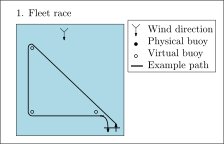
\includegraphics[width=0.6\textwidth]{2019/Challenge_One_EN.pdf}
  \caption{Fleet race challenge requirement}
  \label{fig:fleetrace}
\end{figure}

\subsubsection{Scoring}
A mark/buoy is considered reached if at least one
track point is recorded within a radius of 5m around the position of the
(virtual) buoy.

Teams are scored based on the time between crossing the start line and crossing
the finish line. Teams that do not complete the race will be scored
according to number of markers they reached in the correct order. Teams reaching
the same number of markers will be distinguished based on their time between
crossing the start line and arriving at their last marker. 
The time limit starts counting from the crossing of the start line.

For teams who haven't reach the last way point, the more way points it manage to reach, the higher the rank the team will be.


\subsubsection{Minimum objective}
To be considered for the scoring, the vessel must complete at least the first
leg, from the start line to the first virtual buoy.

\subsection{Station keeping and avoidance}
Sailing robots have a high potential for use as `virtual moorings', maintaining
a fixed position at sea, consuming little energy and without the requirement for
anchoring at the seafloor.
This challenge, consisting of two parts, tests the ship's ability to precisely control in location. 
You need to complete first part 1 before going to the other area to complete part 2 (as shown in the figure). 

\begin{figure}[H]
  \centering
  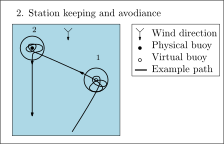
\includegraphics[width=0.6\textwidth]{2019/Challenge_Two_EN.pdf}
  \caption{Station keeping challenge requirement}
  \label{fig:stationkeeping_requirement}
\end{figure}

\paragraph{Part 1}

The station keeping challenge uses a single virtual way point P
(see Figure~\ref{fig:stationkeeping_requirement} part 1). 
After entering a circle with radius $R=15m$ around the way point, the 
sailing vessel aims to stay as close as possible to the way point for 5 minutes.
The challenge is started by releasing the sailing boat at least 20m away
from the waypoint P.


\begin{figure}[H]
  \centering
  \includegraphics[width=0.6\textwidth]{station-keeping}
  \caption{Scoring procedure for the station keeping challenge}
  \label{fig:stationkeeping}
\end{figure}

\paragraph{Part 2}

After finishing the part 1, the boat could continue to take second part of the challenge.
This part of challenge uses a single physical buoy at the centre (see Figure~\ref{fig:stationkeeping_requirement} part 2). 
The GPS coordinate of the physical buoy will be given prior to the start. 
After entering a circle with radius $R=15m$ around the way point, the 
sailing vessel aims to stay as close as possible without touch the buoy for 5 minutes.


\subsubsection{Scoring}

\paragraph{Part 1}

The score is calculated from the positions recorded by a tracker during the 5
minutes after first recording a position within the 15 $m$ radius around P as
follows:
A second point $P_c$ is calculated as the average of the coordinates of all
positions. To be qualified for scoring, the point $P_c$ must be
inside the 15 m circle, regardless of the individual positions.
A circle is fitted around $P_c$, containing 95\% of the positions.
The mean radius of boat trajectory around $P_c$ is $R_{min}$ which is score in part 1.

\paragraph{Part 2}
The score is calculated from the positions recorded by a differential GPS tracker during the 5
minutes after first recording a position within the 15 m radius around physical buoy.
Every touch on the buoy will result in a penalty on the final radius $P_d = \sqrt{1+N}\cdot P_c$,
where $N$ is number of touches. 

Boats are then ranked by the finished parts first. 
Teams finished both parts of challenge is higher ranked than those who finished only one part.
For teams who finished both parts, they ranked by averaged radius in part 1 and 2.
The other teams ranked by the radius in part 1.

%Figure 3 illustrates this procedure. The sailboat track is considered during 5
%minutes after
%entering the red circle (20m radius, centered in the reference waypoint P); the
%average of the
%coordinates of all recorded track points during the 5 mins (green dots) gives
%point Pc; the score
%is calculated with the radius of the blue circle centered in Pc that contains
%95\% of the valid
%track points. 

\subsubsection{Minimum objective}
To be scored in this contest, the vessel must attempt the part 1 and enter the $R=15m$ circle around P
and continue to sail autonomously for five minutes after entering. The resulting 
point $P_c$ must be inside the 15m circle around P.

\subsection{Area scanning}
In recent years, an increasing number of attempts is made at using maritime
vessels in collaboration. A typical
collaborative task is efficiently scanning a large area.
The collaborative area scanning challenge asks teams to take the abilities and
scanning goals of other teams into consideration to optimise their own points.

The scanning task is performed over a large area around the competition, that is
structured in a grid. The boxes of the grid are assigned coordinates. Not all of
the scan area may be suitable for all boats, and it is courtesy of the teams to
choose scan goals suitable for their vessel. The
challenge lasts 60 minutes which teams will be assigned to one of the setup areas
to launch. 

The team can recover their vessels by requesting a safety boat (based on
availability; first come first serve) or by remote controlling the boat from the
pontoon to a start buoy. However, the next attempt must start from the original setup area.
If a team wants to recover the boat, they must first
register the current time with the race committee, so any positions after this
time can be discarded.

During the area scanning challenge, the tracker position is made available 
to all teams live via the tracking website. Teams may update 
highlevel goals (e.g. waypoints) on their vessel remotely or change the software
on the vessel before launching again after a recovery.
Directly controlling the
actuators (e.g. remote control) is not allowed. The race committee may ask to
inspect the code determining updates to the vessel and can apply penalties if
the goal updates are used too excessively.
The boundaries of the scan area, the grid size, and the challenge start- and end time
are announced on the morning of the challenge day.
A bonus can be obtained by providing depth measurements.

\begin{figure}[H]
  \centering
  \includegraphics[width=0.6\textwidth]{2019/Challenge_Three_EN.pdf}
  \caption{Scoring procedure for the station keeping challenge}
  \label{fig:stationkeeping}
\end{figure}


The tracking data of all vessels is available live via the tracking website.

The area scanning challenge starts at the start time, and ends at the end
time given by the race committee on the day. The race committee may split the
challenge into two groups by randomly selecting boats for each group.

\subsubsection{Scoring}

A box in the grid is considered visited by a vessel if at least one track point
of the vessel is registered within that box within the scan time.
One point is available for each box. The first threes teams this get full score, the second team 50~\% and third 33~\%.
Each team receives the final value of all of the boxes that were visited by the
team. 

Boats will be ranked by the final score they achieved from boxes visited by
their vessel.

\subsubsection{Minimum objective}
To be qualified in this challenge, a vessel must register at least one track
point within the scan area during the scan time.

\subsection{Hide and seek}
When operating in a crowded environment, autonomous sailing vessels must be able
recognise and identify each other. 
The hide and seek challenge will evaluate the ability of a sailing boat to dynamic 
track and detect the other boats.

The challenge is competed as a pair with the team ranked close to yours after previous challenges.
For example, first place is paired with second place, third place is paired with fourth place, so on so forth.


  \begin{figure}[H]
    \centering
    \includegraphics[width=0.6\textwidth]{2019/Challenge_Four_EN.pdf}
    \caption{Hide and seek challenge requirement}
    \label{fig:hideandseek}
  \end{figure}

Each team will be assigned to a pair of circles at a diameter of 10 metres (shown as grey and transparent in Figure~\ref{fig:hideandseek}).
Boats may try to \textbf{hide} of \textbf{seek} in this challenge to score points in this challenge.
The \textbf{hide} means sailing in between two circles assigned to your team.
The \textbf{seek} means detect the recognise the other boat while sailing.
Two different A4 size AprilTag will be put on both sides of the sail.
A successful seek would requires the team to take a picture of AprilTag and detect the ID of that tag is situ.
In situ detection means the detection has to done online with the on board processing power. 


\subsubsection{Scoring}

Each successful \textbf{hide} worth one point and \textbf{seek} worth three points.
In this challenge, you can get a maximum 6 points by seeking other boats.
The committee may inspect your \texttt{rosbag} (or your own data recording format) to validate the successful detection. 
Teams are ranked by the total score in this challenge.


\subsubsection{Minimum objective}
To be scored in this challenge, a vessel must enter finished at least one hide or seek. 


\section*{Change log}

\texttt{30-Aug-2019} v1.1 Correct parameters in the competition \\
\texttt{18-June-2019} v1.0 Release and available online

\end{document}

